% A4縦・1段組の学習用（教科書風）
\documentclass[paper=a4,fleqn]{jlreq}
\special{papersize=\the\paperwidth,\the\paperheight}

\usepackage[margin=20truemm]{geometry}
\usepackage[dvipdfmx]{graphicx}
\usepackage{amsmath,amssymb}
\usepackage{tikz}
\usepackage{pgfplots}
\usepackage{etoolbox}
\usepackage{needspace}
\usepackage{bm}
\pgfplotsset{compat=1.18}
\usetikzlibrary{arrows.meta,calc,angles,quotes}

\preto{\section}{\needspace{0.35\textheight}}
\preto{\subsection}{\needspace{0.25\textheight}}

\ModifyHeading{section}{
  lines=1,
  before_space=14pt,
  after_space=6pt
}

\ModifyHeading{subsection}{
  lines=1,
  before_space=10pt,
  after_space=4pt
}

\title{2次元ベクトル}
\author{}
\date{}

\makeatletter
\renewcommand{\maketitle}{%
  \begin{center}
    {\large\bfseries \@title\par}
  \end{center}
  \vspace{4pt}
}
\makeatother

\newcommand{\formula}[1]{%
  \vspace{4pt}%
  \begin{center}{\large\bfseries\boldmath\(\displaystyle #1\)}\end{center}%
  \vspace{4pt}%
}

\begin{document}
\maketitle

\section{ベクトルとは何か}

\subsection{スカラーとベクトル}

数だけを表すものを\textbf{スカラー}という。向きと大きさをまとめて表すものを\textbf{ベクトル}という。

\begin{center}
\begin{tikzpicture}[scale=1.1,>=Stealth]
  \draw[->,gray!70] (-0.4,0) -- (6,0) node[right] {数値の世界};
  \draw[->,gray!70] (-0.4,-1.2) -- (6,-1.2) node[right] {向きのない量};
  \node[draw,rounded corners,fill=gray!10,minimum width=1.7cm,minimum height=0.8cm] at (1.2,-0.3) {8, -3, 5.4};
  \draw[thick,blue,->] (3.3,-0.3) -- (5.3,-0.3) node[midway,above] {右へ};
  \draw[thick,blue,->] (4.2,-0.8) -- (4.2,0.4) node[midway,right] {上へ};
  \node[align=center] at (4.7,-0.3) {ベクトルは\textbf{向き}と\textbf{大きさ}を持つ};
\end{tikzpicture}
\end{center}

\textbf{大事なこと：} ベクトルは「どちらへ」「どれだけ」動くかを1つで表せる。

\subsection{なぜ必要か}

専門学生の学習では、ゲームや図形の計算にそのまま使えることが大事である。ベクトルは位置、速度、押す力、移動方向をまとめて表せるので、考え方がすっきりする。

\textbf{例：}
\begin{itemize}
  \item 右に 2、上に 3 の移動 \(\rightarrow\) \(\vec{v}=\begin{pmatrix}2\\3\end{pmatrix}\)
  \item 斜め左下へ進む力 \(\rightarrow\) 向きと大きさで表す
  \item キャラの速度 \(\rightarrow\) 毎フレームの位置更新に使う
\end{itemize}

\subsection{ベクトルの等しさ}

2つのベクトルが等しいとは、\textbf{大きさが同じ}で\textbf{向きも同じ}ことである。始まる場所は関係ない。

\begin{center}
\begin{tikzpicture}[scale=0.95,>=Stealth]
  \draw[->,gray!60] (-0.5,0) -- (7,0) node[right] {$x$};
  \draw[->,gray!60] (0,-0.5) -- (0,4.2) node[above] {$y$};
  \draw[very thick,blue,->] (0.7,0.8) -- (3.2,2.4);
  \draw[very thick,red,->] (3.8,0.9) -- (6.3,2.5);
  \node[blue] at (1.9,2.65) {$\vec{a}$};
  \node[red] at (5.0,2.7) {$\vec{b}$};
  \node[align=center] at (3.5,0.3) {大きさと向きが同じなら\ $\vec{a}=\vec{b}$};
\end{tikzpicture}
\end{center}

\subsection{確認問題}
\begin{enumerate}
  \item スカラーとベクトルの違いを1文で述べよ。
  \item ベクトルがゲームで使いやすい理由を1つ挙げよ。
  \item 等しいベクトルの条件を答えよ。
\end{enumerate}

\section{成分表示と大きさ}

\subsection{成分表示}

2次元では、ベクトルを横成分と縦成分で表す。

\formula{\vec{a}=\begin{pmatrix}a_x\\a_y\end{pmatrix}}

\begin{center}
\begin{tikzpicture}[scale=1.0,>=Stealth]
  \draw[->,gray!60] (-0.5,0) -- (5.6,0) node[right] {$x$};
  \draw[->,gray!60] (0,-0.5) -- (0,4.4) node[above] {$y$};
  \draw[dashed,gray!60] (0,3) -- (4,3);
  \draw[dashed,gray!60] (4,0) -- (4,3);
  \draw[very thick,blue,->] (0,0) -- (4,3);
  \node[below] at (4,0) {$a_x$};
  \node[left] at (0,3) {$a_y$};
  \node[above right] at (4,3) {$\vec{a}$};
  \node[align=center] at (2.7,1.0) {右に $a_x$、上に $a_y$};
\end{tikzpicture}
\end{center}

\subsection{大きさ}

横と縦を直角三角形の2辺だと思えば、長さはピタゴラスの定理で求められる。

\formula{|\vec{a}|=\sqrt{a_x^2+a_y^2}}

\textbf{例：} \(\vec{a}=\begin{pmatrix}3\\4\end{pmatrix}\) なら、\(|\vec{a}|=5\) である。

\subsection{単位ベクトル}

長さを1にしたベクトルを\textbf{単位ベクトル}という。向きだけを見たいときに使う。

\formula{\hat{a}=\frac{\vec{a}}{|\vec{a}|}}

\subsection{点と点を結ぶベクトル}

点 \(A(x_1,y_1)\) から点 \(B(x_2,y_2)\) へのベクトルは、差をとればよい。

\formula{\overrightarrow{AB}=\begin{pmatrix}x_2-x_1\\y_2-y_1\end{pmatrix}}

\begin{center}
\begin{tikzpicture}[scale=0.95,>=Stealth]
  \draw[->,gray!60] (-0.5,0) -- (6.2,0) node[right] {$x$};
  \draw[->,gray!60] (0,-0.5) -- (0,4.5) node[above] {$y$};
  \coordinate (A) at (1,1);
  \coordinate (B) at (5,4);
  \fill (A) circle (2pt) node[below left] {$A$};
  \fill (B) circle (2pt) node[above right] {$B$};
  \draw[dashed,gray!60] (1,1) -- (5,1) -- (5,4);
  \draw[very thick,blue,->] (1,1) -- (5,4);
  \node at (3.1,2.0) {$\overrightarrow{AB}$};
\end{tikzpicture}
\end{center}

\subsection{確認問題}
\begin{enumerate}
  \item \(\vec{a}=\begin{pmatrix}6\\8\end{pmatrix}\) の大きさを求めよ。
  \item 点 \(A(1,2)\)、点 \(B(4,7)\) のとき、\(\overrightarrow{AB}\) を求めよ。
  \item \(\vec{b}=\begin{pmatrix}-2\\0\end{pmatrix}\) の長さは何か。
\end{enumerate}

\section{ベクトルの足し算と引き算}

\subsection{足し算}

ベクトルの足し算は、成分ごとに足すだけでよい。

\formula{\vec{a}+\vec{b}=\begin{pmatrix}a_x+b_x\\a_y+b_y\end{pmatrix}}

\begin{center}
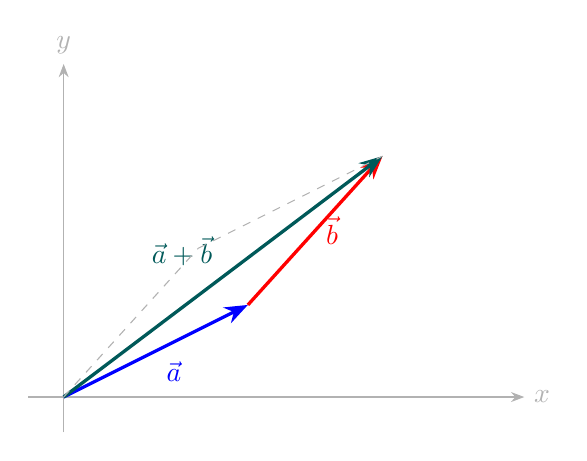
\begin{tikzpicture}[scale=0.9,>=Stealth]
  \draw[->,gray!60] (-0.5,0) -- (6.5,0) node[right] {$x$};
  \draw[->,gray!60] (0,-0.5) -- (0,4.7) node[above] {$y$};
  \coordinate (O) at (0,0);
  \coordinate (A) at (2.6,1.3);
  \coordinate (B) at (4.5,3.4);
  \coordinate (C) at (1.9,2.1);
  \draw[very thick,blue,->] (O) -- (A) node[midway,below right] {$\vec{a}$};
  \draw[very thick,red,->] (A) -- (B) node[midway,right] {$\vec{b}$};
  \draw[very thick,teal!70!black,->] (O) -- (B) node[midway,above left] {$\vec{a}+\vec{b}$};
  \draw[dashed,gray!60] (C) -- (B);
  \draw[dashed,gray!60] (O) -- (C);
\end{tikzpicture}
\end{center}

\subsection{引き算}

引き算は「逆向きのベクトルを足す」と考えると分かりやすい。

\formula{\vec{a}-\vec{b}=\begin{pmatrix}a_x-b_x\\a_y-b_y\end{pmatrix}}

\textbf{例：} \(\begin{pmatrix}5\\2\end{pmatrix}-\begin{pmatrix}2\\3\end{pmatrix}=\begin{pmatrix}3\\-1\end{pmatrix}\)

\subsection{スカラー倍}

数 \(k\) をかけると、ベクトルの長さが \(|k|\) 倍になる。\(k<0\) なら向きも反対になる。

\formula{k\vec{a}=\begin{pmatrix}ka_x\\ka_y\end{pmatrix}}

\begin{center}
\begin{tikzpicture}[scale=0.9,>=Stealth]
  \draw[->,gray!60] (-0.5,0) -- (6.5,0) node[right] {$x$};
  \draw[->,gray!60] (0,-0.5) -- (0,4.7) node[above] {$y$};
  \draw[very thick,blue,->] (0,0) -- (2,1.2) node[midway,above left] {$\vec{a}$};
  \draw[very thick,red,->] (0,0) -- (4,2.4) node[midway,above right] {$2\vec{a}$};
  \draw[very thick,purple,->] (0,0) -- (-2,-1.2) node[midway,below left] {$-\vec{a}$};
\end{tikzpicture}
\end{center}

\subsection{確認問題}
\begin{enumerate}
  \item \(\vec{a}=\begin{pmatrix}1\\2\end{pmatrix}\)、\(\vec{b}=\begin{pmatrix}3\\-1\end{pmatrix}\) のとき、\(\vec{a}+\vec{b}\) を求めよ。
  \item 同じく \(\vec{a}-\vec{b}\) を求めよ。
  \item \(3\vec{a}\) と \(-2\vec{a}\) の意味を言葉で説明せよ。
\end{enumerate}

\section{内積と角度}

\subsection{内積}

2つのベクトルを掛けたとき、結果はスカラーになる。

\formula{\vec{a}\cdot\vec{b}=a_xb_x+a_yb_y}

\textbf{例：} \(\begin{pmatrix}2\\3\end{pmatrix}\cdot\begin{pmatrix}1\\4\end{pmatrix}=2\cdot1+3\cdot4=14\)

\subsection{なす角との関係}

内積は角度とも結びつく。

\formula{\vec{a}\cdot\vec{b}=|\vec{a}||\vec{b}|\cos\theta}

\formula{\cos\theta=\frac{\vec{a}\cdot\vec{b}}{|\vec{a}||\vec{b}|}}

\begin{center}
\begin{tikzpicture}[scale=1.0,>=Stealth]
  \draw[->,gray!60] (-0.5,0) -- (5.8,0) node[right] {$x$};
  \draw[->,gray!60] (0,-0.5) -- (0,4.5) node[above] {$y$};
  \draw[very thick,blue,->] (0,0) -- (4.3,1.3) node[midway,below right] {$\vec{a}$};
  \draw[very thick,red,->] (0,0) -- (3.0,3.4) node[midway,above left] {$\vec{b}$};
  \draw (1.0,0) arc[start angle=0,end angle=35,radius=1.0];
  \node at (1.25,0.45) {$\theta$};
\end{tikzpicture}
\end{center}

\subsection{垂直判定}

\textbf{内積が0なら直角である。}

\formula{\vec{a}\cdot\vec{b}=0 \iff \vec{a}\perp\vec{b}}

\subsection{確認問題}
\begin{enumerate}
  \item \(\vec{a}=\begin{pmatrix}1\\2\end{pmatrix}\)、\(\vec{b}=\begin{pmatrix}3\\1\end{pmatrix}\) の内積を求めよ。
  \item \(\vec{a}=\begin{pmatrix}2\\1\end{pmatrix}\)、\(\vec{b}=\begin{pmatrix}-1\\2\end{pmatrix}\) は垂直か。
  \item なす角が90度のとき、内積はどうなるか。
\end{enumerate}

\section{2次元の外積}

\subsection{2次元の外積はスカラー}

2次元では、外積を\textbf{数}として扱う。向きの判定や面積に使う。

\formula{\vec{a}\times\vec{b}=a_xb_y-a_yb_x}

\textbf{大事：} 正なら反時計回り、負なら時計回りと覚えるとよい。

\begin{center}
\begin{tikzpicture}[scale=1.0,>=Stealth]
  \draw[->,gray!60] (-0.5,0) -- (6.0,0) node[right] {$x$};
  \draw[->,gray!60] (0,-0.5) -- (0,4.7) node[above] {$y$};
  \coordinate (O) at (0,0);
  \coordinate (A) at (4.0,1.0);
  \coordinate (B) at (1.3,3.0);
  \filldraw[fill=blue!8,draw=blue!60] (O) -- (A) -- ($(A)+(B)$) -- (B) -- cycle;
  \draw[very thick,blue,->] (O) -- (A) node[midway,below right] {$\vec{a}$};
  \draw[very thick,red,->] (O) -- (B) node[midway,left] {$\vec{b}$};
  \node at (2.2,1.8) {符号付き面積};
  \draw[->,thick,gray!70] (0.6,0.4) arc[start angle=230,end angle=150,radius=0.5];
  \node at (0.95,0.95) {反時計回り};
\end{tikzpicture}
\end{center}

\subsection{何に使うか}

\begin{itemize}
  \item 3点が左回りか右回りかの判定
  \item 三角形の面積の2倍
  \item 線分どうしの交差判定の補助
\end{itemize}

\subsection{面積との関係}

原点を共有する2本のベクトルがつくる平行四辺形の面積は、外積の絶対値で表せる。

\formula{|\vec{a}\times\vec{b}|=\text{平行四辺形の面積}}

\subsection{確認問題}
\begin{enumerate}
  \item \(\vec{a}=\begin{pmatrix}2\\1\end{pmatrix}\)、\(\vec{b}=\begin{pmatrix}1\\3\end{pmatrix}\) の外積を求めよ。
  \item 外積が正のとき、回転の向きはどうなるか。
  \item 外積の絶対値は何を表すか。
\end{enumerate}

\section{射影}

\subsection{影を落とす考え方}

ベクトルをある方向へ「どれだけ乗っているか」で見るのが\textbf{射影}である。

\formula{\mathrm{proj}_{\vec{b}}\vec{a}=\frac{\vec{a}\cdot\vec{b}}{|\vec{b}|^2}\vec{b}}

\begin{center}
\begin{tikzpicture}[scale=1.0,>=Stealth]
  \draw[->,gray!60] (-0.5,0) -- (6.0,0) node[right] {$x$};
  \draw[->,gray!60] (0,-0.5) -- (0,4.5) node[above] {$y$};
  \draw[very thick,blue,->] (0,0) -- (4.2,3.0) node[midway,above right] {$\vec{a}$};
  \draw[very thick,red,->] (0,0) -- (5.0,0.0) node[midway,below] {$\vec{b}$};
  \draw[dashed,gray!70] (4.2,3.0) -- (4.2,0);
  \draw[very thick,teal!70!black,->] (0,0) -- (4.2,0) node[midway,below] {射影};
  \draw[thin,gray!70] (4.2,3.0) -- (4.2,0);
\end{tikzpicture}
\end{center}

\subsection{意味}

\begin{itemize}
  \item 進行方向にどれだけ成分があるかを見る
  \item 斜めの動きを、横方向・縦方向に分ける
  \item ゲームでは、壁の向きに沿った速度成分を取り出すときに使う
\end{itemize}

\subsection{スカラー射影}

長さだけを取り出したいなら、スカラー射影を使う。

\formula{\frac{\vec{a}\cdot\vec{b}}{|\vec{b}|}}

\subsection{確認問題}
\begin{enumerate}
  \item 射影とは何を表すか。
  \item \(\vec{a}\) を \(\vec{b}\) へ射影するとき、何を使って求めるか。
  \item 斜めの移動を横方向に分けるとき、射影はなぜ便利か。
\end{enumerate}

\section{ゲームで使うベクトル}

\subsection{位置と速度}

ゲームでは、位置の更新をベクトルで書くと整理しやすい。

\formula{\vec{p}(t)=\vec{p}_0+t\vec{v}}

\textbf{例：} 初期位置が \((2,3)\)、速度が \((1,2)\) なら、3秒後は \((5,9)\) になる。

\begin{center}
\begin{tikzpicture}[scale=0.9,>=Stealth]
  \draw[->,gray!60] (-0.5,0) -- (6.5,0) node[right] {$x$};
  \draw[->,gray!60] (0,-0.5) -- (0,5.5) node[above] {$y$};
  \coordinate (P0) at (1,1);
  \coordinate (P1) at (3,3);
  \coordinate (P2) at (5,5);
  \draw[very thick,blue,->] (P0) -- (P1) node[midway,above left] {$\vec{v}$};
  \draw[very thick,red,->] (P1) -- (P2) node[midway,above right] {$\vec{v}$};
  \fill (P0) circle (2pt) node[below left] {$\vec{p}_0$};
  \fill (P1) circle (2pt) node[above left] {$1\text{秒後}$};
  \fill (P2) circle (2pt) node[above right] {$2\text{秒後}$};
\end{tikzpicture}
\end{center}

\subsection{円の衝突判定}

2つの円がぶつかっているかは、中心間の距離で分かる。

\formula{d<r_a+r_b}

\begin{center}
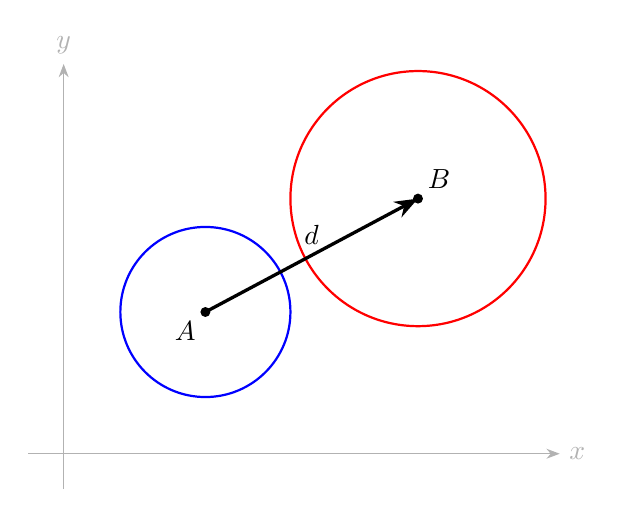
\begin{tikzpicture}[scale=0.9,>=Stealth]
  \draw[->,gray!60] (-0.5,0) -- (7.0,0) node[right] {$x$};
  \draw[->,gray!60] (0,-0.5) -- (0,5.5) node[above] {$y$};
  \coordinate (A) at (2,2);
  \coordinate (B) at (5,3.6);
  \draw[thick,blue] (A) circle (1.2);
  \draw[thick,red] (B) circle (1.8);
  \fill (A) circle (2pt) node[below left] {$A$};
  \fill (B) circle (2pt) node[above right] {$B$};
  \draw[very thick,black,->] (A) -- (B) node[midway,above] {$d$};
\end{tikzpicture}
\end{center}

\subsection{確認問題}
\begin{enumerate}
  \item 速度が \((2,-1)\)、初期位置が \((0,0)\) のとき、2秒後の位置を求めよ。
  \item 半径1の円と半径2の円の中心間距離が2.5なら、衝突しているか。
  \item 射影を使うと、どんなゲーム計算が楽になるか。
\end{enumerate}

\end{document}
